\documentclass[12pt, letterpaper]{memoir}
\usepackage{NotesStyle}
\geometry{margin=0.75in}

\begin{document}
	\mainmatter
	
	\begin{center}
		{\Huge CHEM 3620}
		{\LARGE-- Exam 2 Equations}
		\begin{description}
			\item[Q:] Why does eating a hamburger give you less energy than eating a steak?
		\end{description}
	
		
		\begin{center}
			\begin{equation*}
				\hat{H}\psi = -\dfrac{\hbar^2}{2m}\nabla^2\psi + V\psi = E\psi
			\end{equation*}
		
		
			\begin{minipage}[c]{0.7\textwidth}
				\begin{mdframed}
					\centering
					Spherical Polar Coordinates
					\hrule
					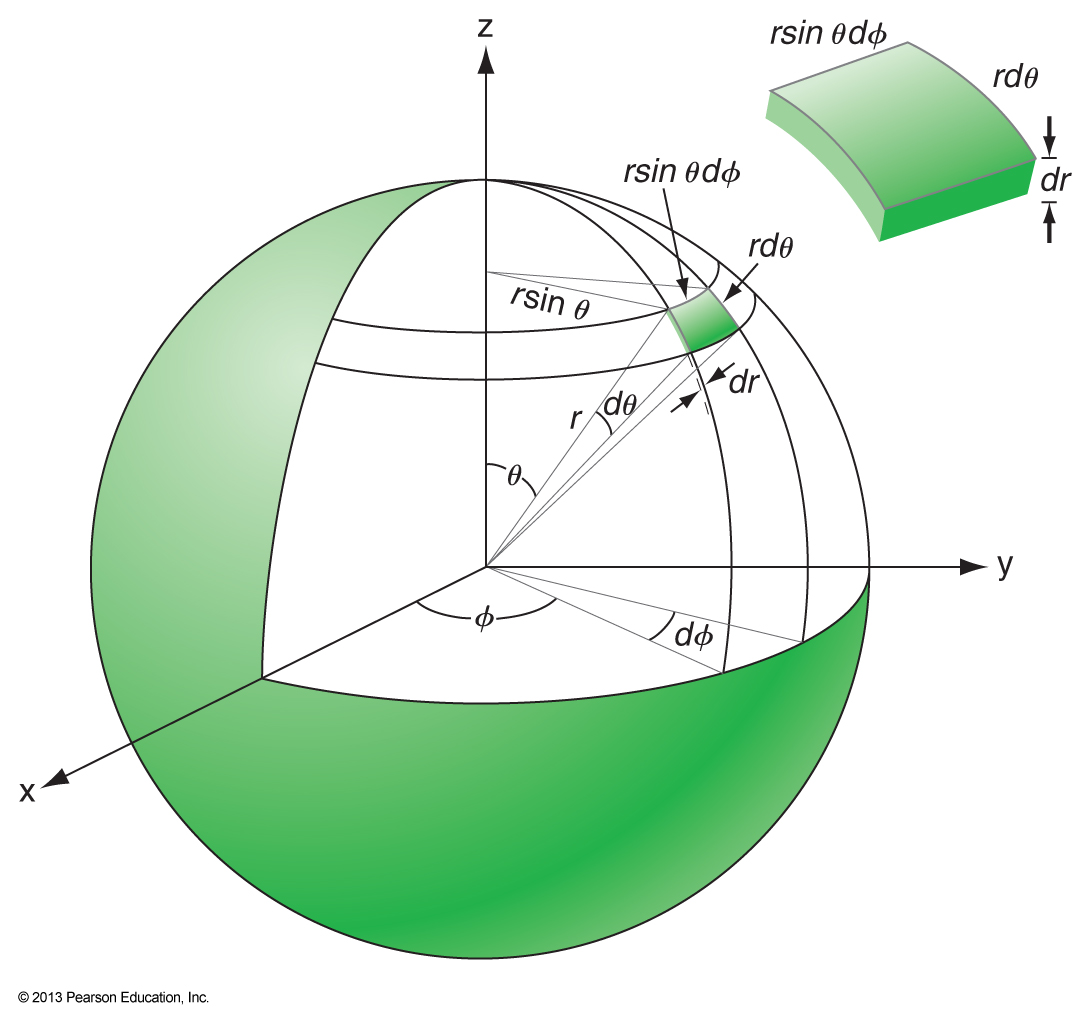
\includegraphics[width = \textwidth]{02_05_Figure}
				\end{mdframed}
			\end{minipage}
		\end{center}

	
		
		\begin{tabular}{ccrl}
			\multicolumn{4}{c}{Table of Particle Properties}\\
			\toprule
			Name&Symbol&\multicolumn{1}{c}{Value}&\multicolumn{1}{c}{Units}\\
			\midrule
			\midrule
			Elementary Charge		& $e$		& $1.602177\times10^{-19}$	& $C$\\
			\midrule
			Electron Rest-Mass		& $m_e$		& $9.109382\times10^{-31}$	& $kg$\\
			\midrule
			Proton Rest-Mass		& $m_p$		& $1.672622\times10^{-27}$	& $kg$\\
			\midrule
			Neutron Rest-Mass		& $m_n$		& $1.674927\times10^{-27}$	& $kg$\\
			\bottomrule
		\end{tabular}

		\begin{description}
			\item[A:] Because hamburger is the ground state of beef.
		\end{description}
		
				
	\end{center}
	
	\newpage

		\begin{minipage}{0.45\textwidth}
			
			\begin{equation*}
				\tilde{\nu}=\tilde{R}_H\left(\dfrac{1}{n_1^2}-\dfrac{1}{n_2^2}\right)
			\end{equation*}
			
			\begin{equation*}
				\tilde{R}_H=109677~cm^{-1}
			\end{equation*}
			
			\begin{equation*}
				P(r)=r^2\left|R(r)\right|^2
			\end{equation*}
			
			\begin{equation*}
				\tilde{\nu} = E_{KE} + \phi
			\end{equation*}
			
			\begin{equation*}
				\chi = \frac{1}{2}\left(I + E_{ea}\right)
			\end{equation*}
			
			\begin{equation*}
				E_\pm = \dfrac{\alpha\pm\beta}{1\pm S}
			\end{equation*}
			
			\begin{equation*}
				c_A=\dfrac{1}{\sqrt{2(1\pm S)}}
			\end{equation*}
			
			\begin{equation*}
				c_A = \left[1+\left(\dfrac{\alpha_A-E}{\beta}\right)^2\right]^{-\nicefrac{1}{2}}
			\end{equation*}
			
			\begin{equation*}
				h = 6.626\times10^{-34}J~s
			\end{equation*}
		
		\end{minipage}
		\begin{minipage}{0.54\textwidth}	
			
			\begin{equation*}
				\tilde{\nu}=\dfrac{1}{\lambda\left(cm\right)}=\dfrac{\nu}{c\left(\nicefrac{cm}{s}\right)}}
			\end{equation*}
			
			\begin{equation*}
				R_{n,l}(r) = N_{n,l}\rho^lL_{n-l-1}^{2l+1}(\rho)e^{-\nicefrac{\rho}{2}}
			\end{equation*}
			
			\begin{equation*}
				\mu_{jk}=\displaystyle\int \psi_j^*\hat{\mu}\psi_k\mathrm{d}\tau
			\end{equation*}
			
			\begin{equation*}
				\psi = c_A\chi_A + c_B\chi_B
			\end{equation*}
			
			\begin{equation*}
				\left|\chi_A-\chi_B\right| = \left[D_0(AB)-\frac{1}{2}\left(D_0(AA)+D_0(BB)\right)\right]^{\nicefrac{1}{2}}
			\end{equation*}
			
			\begin{equation*}
				E_\pm = \frac{1}{2}\left(\alpha_A+\alpha_B\right) \pm\frac{1}{2}\left(\alpha_A-\alpha_B\right) \left[1+\left(\dfrac{2\beta}{\alpha_A-\alpha_B}\right)^2\right]^{\nicefrac{1}{2}}
			\end{equation*}
			
			\begin{equation*}
				c_B = \pm c_A
			\end{equation*}
			
			\begin{equation*}
				c_B = \left[1+\left(\dfrac{\beta}{\alpha_A-E}\right)^2\right]^{-\nicefrac{1}{2}}
			\end{equation*}
			
			\begin{equation*}
				\hbar = 1.055\times10^{-34}J~s
			\end{equation*}
		\end{minipage}

\end{document}	